\section{方程类型}
\label{sec:pdeprob-types}

Poisson方程、热方程和波动方程都是二阶线性方程，需要的数据却不同，传播信息的方式也不同。能否不解方程，只看系数就把它们区分开？

\paragraph{主部与高频响应}
记自变量为$\bm{z}\in\mathbb{R}^{N}$，二阶线性方程写成
\begin{equation}
  \sum_{i,j=1}^{N}M_{i,j}(\bm{z})\,\partial_{z_i}\partial_{z_j}u+(\text{一阶及零阶项})=f,
  \label{eq:pdeprob-second-order}
\end{equation}
其中$\bm{M}(\bm{z})$是实对称矩阵。对称性不是限制：混合偏导相等，$M_{i,j}$与$M_{j,i}$只有两者之和起作用，可以都换成平均值。二阶项的全体称为方程的\term{主部}（principal part）。

为什么分类只看主部？在一点附近把系数看成常数，代入高频振荡$u=\mathrm{e}^{\mathrm{i}\bm{\xi}\cdot\bm{z}}$。二阶项给出因子$-\bm{\xi}^{\top}\bm{M}\bm{\xi}$，大小与$\lVert\bm{\xi}\rVert_2^{2}$同阶，一阶项只有$\lVert\bm{\xi}\rVert_2$的量级。频率越高，主部越占支配地位。

所以方程对高频振荡的反应由二次型$\bm{\xi}^{\top}\bm{M}\bm{\xi}$决定。若对所有非零$\bm{\xi}$它都不为零，任何方向的高频振荡都会被主部放大成很大的量，无法存在于解中，除非右端也这样振荡；若沿某个方向它等于零，主部感觉不到沿这个方向的振荡，这种振荡就可以在解中传播。二次型的性质由$\bm{M}$的特征值的符号决定。

\begin{definition}[二阶线性方程的类型]
\label{def:pdeprob-types}
设$\bm{M}(\bm{z})$是式~\eqref{eq:pdeprob-second-order}在点$\bm{z}$处的系数矩阵。根据它的特征值，称方程在该点是
\begin{enumerate}
  \item \term{椭圆型}（elliptic）：全部特征值非零且同号；
  \item \term{抛物型}（parabolic）：恰有一个特征值为零，其余同号，且相应零特征方向上有一阶项；
  \item \term{双曲型}（hyperbolic）：全部特征值非零，且恰有一个的符号与其余相反。
\end{enumerate}
\end{definition}

这三类并不穷尽所有情形。$N\geq4$时可以有两正两负的特征值，例如下面的方程不属于这三类：
\[
  \partial_{z_1}^{2}u+\partial_{z_2}^{2}u-\partial_{z_3}^{2}u-\partial_{z_4}^{2}u=0.
\]

抛物型的定义中要求一阶项，是因为把$\partial_x^{2}u=0$看成$(x,t)$的方程时，$\bm{M}$也有零特征值，但其中$t$只是参数，方程实质上是关于$x$的常微分方程。

把四个模型代入。Poisson方程的$\bm{z}=\bm{x}$，$\bm{M}=-\bm{I}$，椭圆型。热方程的$\bm{z}=(\bm{x},t)$，
\[
  \bm{M}=\operatorname{diag}(-1,\ldots,-1,0),
\]
零特征方向是时间方向，那里有一阶项$\partial_tu$，抛物型。波动方程的$\bm{z}=(\bm{x},t)$，
\[
  \bm{M}=\operatorname{diag}(-c^{2},\ldots,-c^{2},1),
\]
恰有一个特征值与其余反号，双曲型。输运方程是一阶方程，没有二阶项，不在这个分类中。

两个变量时分类有一个常用的判别式。考虑方程
\[
  a_1\partial_y^{2}u+2a_2\partial_y\partial_zu+a_3\partial_z^{2}u+(\text{低阶项})=f.
\]
它的系数矩阵的行列式是$a_1a_3-a_2^{2}$，也就是两个特征值之积。于是$a_2^{2}-a_1a_3$小于零、等于零、大于零分别对应椭圆、抛物、双曲型（抛物型另需一阶项）。

名称来自把$\partial_x$换成$\xi$、把$\partial_t$换成$\tau$后得到的曲线，如图~\ref{fig:pdeprob-conics}：二维Laplace算子给出$\xi^{2}+\tau^{2}=1$，热算子给出$\tau=\xi^{2}$，波动算子给出$\tau^{2}-\xi^{2}=1$。这只解释了名字的来历，真正起作用的是下面要讲的传播方式。

\begin{BookInlineFigure}
  \centering
  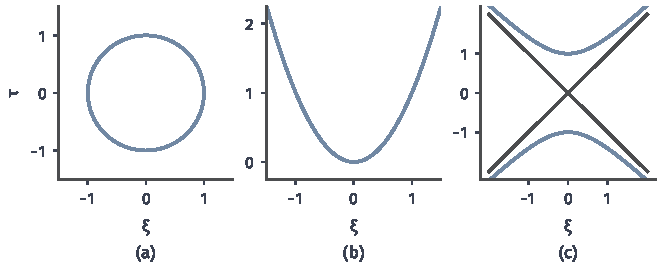
\includegraphics[width=112.0mm]{figures/06-differential-equations/02-partial-differential-equations/matplotlib/pdeprob-conics/figure.pdf}
  \caption{三类方程名称的来历。(a)椭圆$\xi^2+\tau^2=1$。(b)抛物线$\tau=\xi^2$。(c)双曲线$\tau^2-\xi^2=1$，深灰直线是渐近线$\tau=\pm\xi$，它们对应二次型为零的方向。}
  \label{fig:pdeprob-conics}
\end{BookInlineFigure}

\paragraph{分类不依赖坐标}
类型只有在换坐标后不变才有意义。下面的引理说明它只依赖特征值符号的个数。

\begin{lemma}[类型在坐标变换下不变]
\label{lem:pdeprob-invariance}
设$\bm{y}=\bm{\Phi}(\bm{z})$是二阶连续可微的可逆坐标变换，其Jacobi矩阵$\bm{J}$处处可逆。在新坐标下，式~\eqref{eq:pdeprob-second-order}的系数矩阵是
\begin{equation}
  \widetilde{\bm{M}}=\bm{J}\bm{M}\bm{J}^{\top},
  \label{eq:pdeprob-congruence}
\end{equation}
且$\widetilde{\bm{M}}$与$\bm{M}$的正、负、零特征值个数分别相同。
\end{lemma}

\begin{proof}
记$\widetilde{u}(\bm{y})=u(\bm{z})$。由链式法则，
\[
  \partial_{z_i}u=\sum_{k}J_{k,i}\,\partial_{y_k}\widetilde{u}.
\]
再求一次导数，二阶导数项来自对$\partial_{y_k}\widetilde{u}$求导，对$J_{k,i}$求导只产生一阶项，于是
\[
  \partial_{z_i}\partial_{z_j}u=\sum_{k,l}J_{k,i}J_{l,j}\,\partial_{y_k}\partial_{y_l}\widetilde{u}+(\text{一阶项}).
\]
代入式~\eqref{eq:pdeprob-second-order}，$\partial_{y_k}\partial_{y_l}\widetilde{u}$的系数是$\sum_{i,j}J_{k,i}M_{i,j}J_{l,j}$，这就是式~\eqref{eq:pdeprob-congruence}。

$\bm{M}$的正特征值个数等于使二次型在其上正定的子空间的最大维数。变量替换$\bm{\xi}=\bm{J}^{\top}\bm{\eta}$是线性双射，把$\bm{M}$的这类子空间一一映成$\widetilde{\bm{M}}$的这类子空间，维数不变。负特征值同理，零特征值的个数由总数$N$确定。
\end{proof}

\paragraph{特征方向}
引理还回答了哪些曲面特殊。设曲面由$\varphi(\bm{z})=$常数给出，$\nabla_{\bm{z}}\varphi\neq\bm{0}$。若把$\varphi$取作新坐标$y_1$，$\bm{J}$的第一行就是$(\nabla_{\bm{z}}\varphi)^{\top}$，由式~\eqref{eq:pdeprob-congruence}，
\[
  \widetilde{M}_{1,1}=(\nabla_{\bm{z}}\varphi)^{\top}\bm{M}\,\nabla_{\bm{z}}\varphi.
\]
若这个量为零，新方程中不含$\partial_{y_1}^{2}\widetilde{u}$，方程就无法用曲面上的值和一阶法向导数算出二阶法向导数。这样的曲面称为\term{特征曲面}（characteristic surface），两个自变量时称为\term{特征线}（characteristic curve）。二阶法向导数穿过它可以有跳跃，解的不光滑性可以沿它存在。

下面用一个可以手算的方程走一遍。考虑
\[
  \partial_y^{2}u+4\partial_y\partial_zu+3\partial_z^{2}u=0.
\]
这里$a_1=1$，$a_2=2$，$a_3=3$，判别式$a_2^{2}-a_1a_3=1>0$，方程是双曲型。系数矩阵的两个特征值是$2\pm\sqrt{5}$，确实异号。

把算子分解为两个一阶因子，
\[
  \partial_y^{2}+4\partial_y\partial_z+3\partial_z^{2}=(\partial_y+\partial_z)(\partial_y+3\partial_z).
\]
第一个因子把任何$\psi(y-z)$变成零，第二个因子把任何$\varphi(3y-z)$变成零，因此方程的通解是
\[
  u(y,z)=\varphi(3y-z)+\psi(y-z).
\]
验证特征条件：取$\varphi_1=y-z$，梯度$(1,-1)^{\top}$代入二次型得$1-4+3=0$；取$\varphi_2=3y-z$，梯度$(3,-1)^{\top}$代入得$9-12+3=0$。解确实由沿这两族直线传播的两个函数组成。

三个模型的特征曲面反映了各自的传播方式。对Poisson方程，$\bm{M}=-\bm{I}$，二次型只在零向量上为零，没有特征曲面。对热方程，$\nabla\varphi$必须只有时间分量，特征曲面是水平的$t=$常数。对一维波动方程，二次型$\tau^{2}-c^{2}\xi^{2}$的零点给出直线$x\pm ct=$常数。

\paragraph{类型决定传播方式}
图~\ref{fig:pdeprob-dependence}用一个内部点$P$说明三种类型的依赖关系。椭圆型中，$P$处的值受整个边界影响，没有时间方向，也没有“上游”。抛物型中，$P$处的值依赖此前全部时刻的整个区域；特征面水平，信息在同一时刻立刻到达各处。双曲型中，$P$处的值只依赖向过去张开的一个圆锥。

\begin{BookInlineFigure}
  \centering
  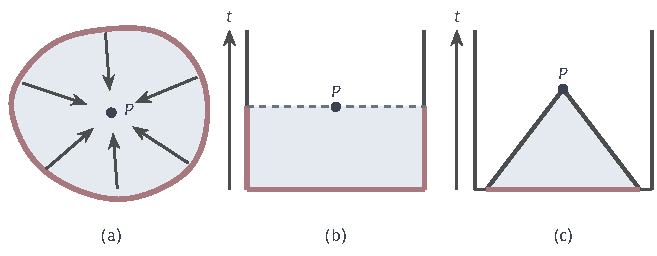
\includegraphics[width=111.3mm]{figures/06-differential-equations/02-partial-differential-equations/tikz/pdeprob-dependence/figure.pdf}
  \caption{内部点$P$的值依赖哪些数据（红）。(a)椭圆型：整个边界都影响$P$。(b)抛物型：时空图中，$P$之前的全部初值和侧面边值都影响$P$，浅蓝部分为依赖区域。(c)双曲型：只有深灰特征线所夹的底边影响$P$，这段红色底边之外的初值不起作用。}
  \label{fig:pdeprob-dependence}
\end{BookInlineFigure}

用点刺激可以把这种差别算出来。把总量为$1$的源或初值集中到一点，看三个方程的响应。在$(0,1)$上，两端为零、中点受单位点源的Poisson解是
\[
  u(x)=\frac12\min\{x,1-x\},
\]
它是一条折线，折点处斜率由$1/2$跳到$-1/2$，跳跃量$1$正好是点源的强度。解在整个区间上都不为零。

实轴上的热方程从原点的单位点热源出发，解是
\begin{equation}
  G(x,t)=\frac{1}{\sqrt{4\pi t}}\exp\Bigl(-\frac{x^{2}}{4t}\Bigr),\qquad t>0.
  \label{eq:pdeprob-heat-kernel}
\end{equation}
直接求导可以验证它满足方程：
\[
  \partial_tG=\partial_x^{2}G=\Bigl(\frac{x^{2}}{4t^{2}}-\frac{1}{2t}\Bigr)G.
\]
对任意$t>0$和任意$x$都有$G>0$，影响瞬间到达每一点，只是远处非常小。例如$x=1$，$t=0.01$时，$G\approx3.9\times10^{-11}$。

实轴上的波动方程以$c=1$、初位移为零、初速度为单位点刺激时，解是
\[
  u(x,t)=\frac12\mathbb{I}\{\lvert x\rvert<t\},
\]
影响的前沿以速度$1$前进，前沿之外严格为零。图~\ref{fig:pdeprob-point-response}并排画出了这三种响应。

\begin{BookInlineFigure}
  \centering
  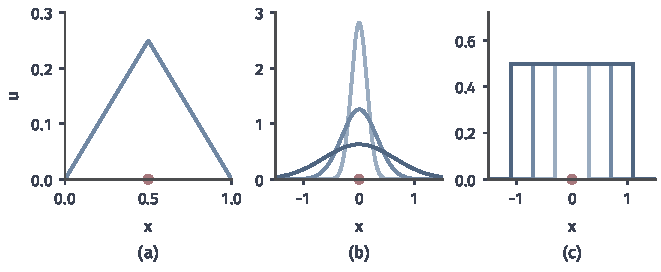
\includegraphics[width=112.0mm]{figures/06-differential-equations/02-partial-differential-equations/matplotlib/pdeprob-point-response/figure.pdf}
  \caption{对单位点刺激（红点）的响应。(a)$(0,1)$上的Poisson方程，解为折线。(b)实轴上的热方程，蓝色由浅到深为$t=0.01,0.05,0.2$，处处为正。(c)实轴上的波动方程，$c=1$，蓝色由浅到深为$t=0.3,0.7,1.1$，前沿之外为零。}
  \label{fig:pdeprob-point-response}
\end{BookInlineFigure}

表~\ref{tab:pdeprob-type-roles}汇总了这些差别，以及与之相配的数据。表中的结论是对模型方程而言的典型行为，一般方程要在相应条件下分别证明。

\begin{BookInlineTable}
  \centering
  \begin{tabular}{llll}
    \toprule
     & 椭圆型 & 抛物型 & 双曲型\\
    \midrule
    模型 & Poisson & 热 & 波动\\
    数据 & 全部边界 & 初值、侧面 & 两个初值、侧面\\
    传播 & 无时间方向 & 速度无穷 & 速度有限\\
    不光滑性 & 内部不产生 & 瞬间抹平 & 沿特征传播\\
    时间方向 & 无 & 不可逆 & 可逆\\
    \bottomrule
  \end{tabular}
  \caption{三类二阶模型方程的典型行为。}
  \label{tab:pdeprob-type-roles}
\end{BookInlineTable}

\paragraph{分类的适用范围}
类型是逐点定义的，系数随位置变化时类型可以改变。Tricomi方程$y\,\partial_x^{2}u+\partial_y^{2}u=0$的系数矩阵是$\operatorname{diag}(y,1)$：$y>0$时椭圆型，$y<0$时双曲型，$y=0$时退化。

在$y<0$的半平面，特征线满足$y\varphi_x^{2}+\varphi_y^{2}=0$，取$\varphi=x\mp\frac23(-y)^{3/2}$可以直接验证。图~\ref{fig:pdeprob-tricomi}中这两族曲线在下半平面交织，在$y=0$处形成尖点，上半平面没有特征线。这样的方程要在两个区域上分别提数据，不能套用单一类型的结论。

\begin{BookInlineFigure}
  \centering
  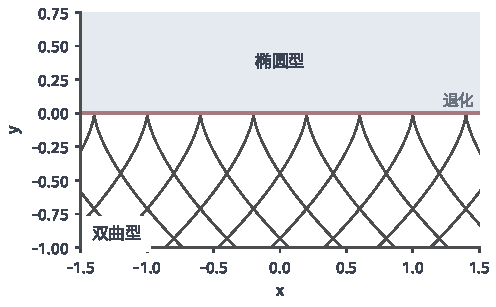
\includegraphics[width=84.0mm]{figures/06-differential-equations/02-partial-differential-equations/matplotlib/pdeprob-tricomi/figure.pdf}
  \caption{Tricomi方程$y\,\partial_x^2u+\partial_y^2u=0$的类型随位置变化。上半平面（浅蓝）椭圆型，红线$y=0$处退化，下半平面双曲型，深灰曲线是特征线$x\mp\frac23(-y)^{3/2}=$常数。}
  \label{fig:pdeprob-tricomi}
\end{BookInlineFigure}

分类也不记录变量的角色。方程$\partial_tu=\partial_x^{2}u$把$t$换成$-t$，得到$-\partial_tu=\partial_x^{2}u$，$\bm{M}$完全相同，仍是抛物型。但第一个方程向未来演化是好问题，向过去演化却不是，第~\ref{sec:pdeprob-well-posedness}节将具体算出差别。所以说一个方程是抛物型时，还要说明哪个变量是时间、沿哪个方向演化。

拟线性方程的主部系数依赖解，类型要在给定的解处判断，同一方程对不同的解可以不同。分类本身是线性方程的概念，推广到非线性方程总要先指明在哪个解上取线性化。

\paragraph{一阶方程按特征传播}
一阶方程没有二阶主部，二次型的分类对它们说不出什么，要改用另一种语言：信息沿曲线传递，这些曲线由常微分方程确定，同样称为特征线。

输运方程$\partial_tu+\bm{v}\cdot\nabla u=0$的特征线就是流体粒子的轨迹$\mathrm{d}\bm{x}/\mathrm{d}t=\bm{v}(\bm{x},t)$，它由给定的速度场决定，与解无关，沿线$u$不变。

非线性时情况改变。守恒律$\partial_tu+\partial_xF(u)=0$可以写成$\partial_tu+F'(u)\partial_xu=0$，信息的传播速度$F'(u)$依赖解本身，不同位置出发的曲线可能相交。Hamilton--Jacobi方程$\partial_tu+H(\nabla u)=0$对梯度非线性，沿曲线传递的是值和梯度，解在曲线相遇处会产生尖点。

这些方程的中心问题不是分类，而是相交之后如何选择解。这需要先搞清楚“解”究竟是什么意思。
